\documentclass{beamer}
\beamertemplatenavigationsymbolsempty
\setbeamercolor{block title}{use=structure,fg=white,bg=structure!50}
\setbeamercolor{block body}{parent=normal text,use=block title,bg=black!5}

\usepackage{listings}
\lstset{basicstyle=\scriptsize\tt}
\lstset{keywordstyle=\scriptsize\bf}

\author{Florian Schanda}
\title{What is MISS\_HIT}

\begin{document}

\maketitle

\begin{frame}{Overview}
  \structure{MISS\_HIT} is:
  \begin{itemize}
  \item A feature-complete free-software lexer and parser for GNU MATLAB\texttrademark\ and Octave
    \pause
  \item A supplementary tool-suite for MATLAB\texttrademark\ and GNU
    Octave
    \begin{itemize}
    \item A \structure{style checker}
    \item A \structure{code formatter}
    \item A \structure{code metric tool}
    \end{itemize}
  \end{itemize}
\end{frame}

\begin{frame}{Availability, License, and Requirements}
  \begin{itemize}
  \item Available on GitHub: \url{https://github.com/florianschanda/miss_hit}
  \item Licensed under GPLv3
  \item Requires only Python 3.6+
  \item Does \emph{not} require a working MATLAB\texttrademark\ or GNU
    Octave environment
  \end{itemize}
\end{frame}

\begin{frame}{Tool overview}{Style checker}
  \begin{itemize}
  \item Can check many style issues, e.g:
    \begin{itemize}
    \item Whitespace issues
    \item Indentation
    \item Naming of variables, functions, classes
    \item etc.
    \end{itemize}
  \end{itemize}
\end{frame}

\begin{frame}[fragile]{Tool overview}{Style checker}
  \begin{block}{Example code}
\begin{lstlisting}[language=MATLAB]
if (foo)
\end{lstlisting}
  \end{block}
  \pause
  \begin{block}{Output of mh\_style.py}
    \scriptsize
\begin{verbatim}
In test.m, line 7
| if (foo)
|    ^ style: redundant parenthesis
\end{verbatim}
  \end{block}
\end{frame}

\begin{frame}{Tool overview}{Code formatter}
  \begin{itemize}
  \item Almost all issues can be automatically fixed
  \item Just use the {\tt --fix} option
  \end{itemize}
\end{frame}

\begin{frame}[fragile]{Tool overview}{Code formatter}
  \begin{block}{Example code}
\begin{lstlisting}[language=MATLAB]
function rv= foo (x), if x < 0,,rv=-x;else,rv=x;,; end;
\end{lstlisting}
  \end{block}
  \pause
  \begin{block}{Fixed code using mh\_style.py --fix}
\begin{lstlisting}[language=MATLAB]
function rv = foo (x)
    if x < 0
        rv = -x;
    else
        rv = x;
    end
\end{lstlisting}
  \end{block}
\end{frame}

\begin{frame}[fragile]{Tool overview}{Code formatter}
  Code formatter is fully aware of all whitespace peculiarities!
  \pause
  \begin{itemize}
  \item \verb|[1 1]|
  \item \verb|[1+1]|
  \item \verb|[1+ 1]|
  \item \verb|[1 +1]|
  \item \verb|[1 + 1]|
  \item \verb|[1 ++ 1]|
  \item \verb|[1 + + 1]|
  \item \verb|[1+ +1]|
  \end{itemize}
  All of this works correctly!
\end{frame}

\begin{frame}{Tool overview}{Code metric tool}
  MISS\_HIT also includes a code metric tool that can measure:
  \begin{itemize}
  \item Cyclomatic complexity (equivalent to {\tt mlint})
  \item Path count
  \item Maximum nesting of control structures
  \item Number of function parameters
  \item Number of global variables
  \item Number of persistent variables
  \item Line count for each function
  \end{itemize}
\end{frame}

\begin{frame}{Tool overview}{Code metric tool}
  HTML report is probably the most useful:
  \begin{center}
    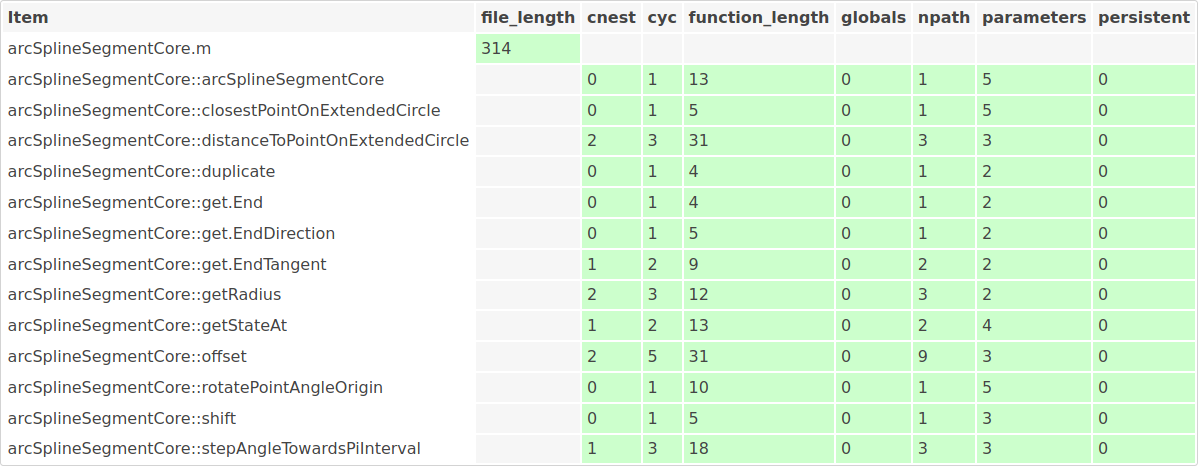
\includegraphics[width=10cm]{metrics.png}
  \end{center}
\end{frame}

\begin{frame}[fragile]{Tool overview}{Code metric tool}
  Exceeding metric generates errors!
  \begin{block}{Example}
    \scriptsize
\begin{verbatim}
In function_file.m, line 3
| function function_file
|          ^^^^^^^^^^^^^ metric: exceeded npath: measured 8 > limit 5
\end{verbatim}
  \end{block}
\end{frame}

\begin{frame}[fragile]{Tool overview}{Code metric tool}
  Justification mechanism allows you to locally exceed limits:
\begin{block}{Justification pragma example}
\begin{lstlisting}[language=MATLAB]
function function_file_justified
  %| pragma Justify(metric, "npath",
  %|                "this is fine for reasons...");
  if rand() > 0.5
    disp heads;
  else
    disp tails;
  end

  % ...
\end{lstlisting}
\end{block}
\end{frame}

\begin{frame}{Optimised for CI}
  MISS\_HIT is ideal for integration in your continuous integration
  environment:
  \begin{itemize}
  \item Low foot-print, no requirements (only Python 3)
  \item Multi-threaded analysis
  \item Justification mechanism allows you to maintain code metrics
    and style on every commit
  \item When it comes to ``release'' time, you just need to generate
    reports and you're done
  \end{itemize}
\end{frame}

\begin{frame}{Getting help}
  \begin{itemize}
  \item Documentation describes everything: style rules, metrics, and
    how to use the configuration files
  \item \url{https://florianschanda.github.io/miss_hit/}
  \item Found a bug / want something done? Raise an issue on GitHub!
  \end{itemize}
\end{frame}

\begin{frame}{Possible ideas for MISS\_HIT}
  Some ideas for the future:
  \begin{itemize}
  \item Analyze embedded code inside SIMULINK\texttrademark\ models
  \item Linter tool
  \item More Octave support
  \item Octave / MATLAB\texttrademark\ compatibility check
  \item Tool qualification for e.g. ISO 26262
    \pause
  \item \structure{Anything else users suggest!}
  \end{itemize}
\end{frame}

\end{document}
